\chapter[P2: A Logical Beginning]{P2: A Logical Beginning}
\label{ch:p2}

Our journey begins at U.C.~Berkeley in $2003$, where just beyond the protests
at Sproul Plaza, the Declarative Networking project was just getting underway.
The project would see the development of a new declarative language called {\em
\OVERLOG} and its companion runtime {\em P2}.  The aim was to make it easy to
implement and deploy overlay networks by allowing specifications in a
high-level declarative language to be directly executed on nodes that span the
Internet.  These overlay specifications, expressed as \OVERLOG rules, contained
{\em orders of magnitude} fewer lines of code than corresponding overlay
implementations written in an imperative language (e.g., C/C++).  The project
implemented, and deployed, declarative versions of a Narada-style mesh
network~\cite{chu00case}, using only 12 ``rules'', and the Chord structured
overlay~\cite{chord} in only 35 ``rules''~\cite{p2:sosp}, versus thousands of
lines of C code for the MIT Chord reference implementation.  From the many
contributions made during its tenure, the Declarative Networking project showed
that relations, together with a recursive query language, can fairly naturally
represent the persistent routing state of the overlays it
considered~\cite{boon-thesis}.

The \OVERLOG language is a descendent of Datalog, which we introduce in
Section~\ref{ch:p2:sec:datalog}.  In Section~\ref{ch:p2:sec:overlog} we present
the \OVERLOG language by detailing its extensions to Datalog: it adds a
notation to specify the location of data, provides some SQL-style extensions
such as primary keys and aggregation, and it defines a new model for processing
and generating changes to tables.  Section~\ref{ch:p2:sec:p2} describes the P2
runtime, which is responsible for compiling and executing \OVERLOG programs on
a set of distributed nodes.  The design of P2 was inspired by prior work in
both databases and networking.  It is based in large part upon a side-by-side
comparison of the PIER peer-to-peer query engine~\cite{pier-cidr05} and the
Click modular router~\cite{click-tocs}.  Like PIER, P2 can manage structured
data tuples flowing through a broad range of query processing elements, which
may accumulate significant state and perform substantial asynchronous
processing.  Like Click, P2 stresses high-performance transfers of data units,
as well as dataflow elements with both ``push'' and ``pull'' modalities.  We
conclude this chapter in Section~\ref{ch:p2:sec:summary} with a summary of the
``networking'' portion of the Declarative Networking project before presenting
its final Chapters~\ref{ch:evita}, \ref{ch:magic} and~\ref{ch:opt}.

\section{Introduction to Datalog}
\label{ch:p2:sec:datalog}

This discussion on Datalog follows from the description in Ramakrishnan and
Ullman's survey~\cite{deductive-database}, and the many superb course
notes~\cite{ullmanNotes} on the subject.  Datalog drew inspiration from the
Prolog language, which was one of the first logic programming languages.  Both
Datalog and Prolog consist of a set of declarative {\em rules} and an optional
{\em query}.  A rule has the form $p\ \text{\ol{:-}}\ q_1,\ q_2,\ \ldots,\
q_n$, which represents a disjunction of literals.  Informally, a rule reads
''{\bf if} $q_1$ and $q_2$ and $\ldots$ and $q_n$ is true {\bf then} $p$ is
true``.  Literals are either {\em predicates} over {\em fields} (variables and
constants), or function symbols applied to fields.  The predicate appearing to
the left of the \ol{:-} symbol is the head predicate, and those to the right
are body predicates or ``subgoals.'' Recursion is expressed by rules that refer
to each other in a cyclic fashion.  That is, the head predicate also appears as
a subgoal in the rule, or indirectly through some other.

A predicate literal is a named reference to a set of data tuples associated
with a specific schema.  In Datalog, a data tuple is referred to as fact, which
is stored in a relational table, that may not necessarily fit in memory.  Two
common notions are used when referring to the predicates that appear in a
Datalog program.  A predicate whose relation is stored in the database is
called an {\emph extensional database} (EDB) relation, while those that are
defined by logical rules are called {\emph intensional database} (IDB)
relations.  In other words, EDB tuples are those that persist in the database
as relations, while IDB predicates are more like ``views'' (or stored queries)
over the database schema.

During evaluation, EDB facts represent the input to the Datalog program, and
IDB derivations are the output.  Datalog, unlike Prolog, evaluates its rules in
a bottom up fashion, starting with all known EDB facts, and deriving new IDB
facts through rule deductions.  A key consequence of a bottom-up evaluation
strategy is that it can efficiently handle ``large data'' sets, whose size well
exceeds the capacity of a machine's main memory.  Prolog on the other hand uses
a top-down evaluation approach that precludes the efficient use of relational
operators (i.e., select, project, join).  As a further result, Prolog's state
is confined to the main memory boundaries of the running system, since its
``graph'' based algorithm requires all facts be accounted for at once.

\subsection{Safety First}

There are constraints that must be in place for a Datalog program to make sense
as operations on finite relations.  A {\emph safe} Datalog rule is one that
restricts the range of all variables appearing in the head by ensuring that
each such variable appear as a field in some predicate(s) of the rule body.
For example, the following rule is not safe since it does not restrict the $P$
variable in the \ol{path} head predicate.

\begin{minipage}{\linewidth}
\ssp
{\bf path}(X, Y, P, C) :- {\bf link}(X, Y, C). \\
\end{minipage}
The above rule generates an infinite number of \ol{path} tuples since we can
substitute $P$ with any list of strings (for example).  This ``safety''
restriction imposed by Datalog semantics ensures that a finite (IDB) solution is
obtained from applying a finite set of rules to a finite (EDB) input.  Datalog
further restricts its (IDB) output to set semantics, as opposed to bag
semantics that allow duplicate tuples.  The reader can assume these safe restrictions
in all the rules presented in this thesis.

\subsection{Our first Datalog Program}

\begin{figure*}
\ssp
\begin{boxedminipage}{\linewidth}
{\bf link}(``node1'', ``node2'', 1). \\
{\bf link}(``node2'', ``node3'', 1). \\
\\
R1 {\bf path}(X, Y, {\em cons}(X, Y), C) :- \\
\datalogspace {\bf link}(X, Y, C). \\
\\       
R2 {\bf path}(X, Z, {\em cons}(X, P2), C1+C2) :- \\
\datalogspace {\bf link}(X, Y, C1), {\bf path}(Y, Z, P2, C2), \\
\datalogspace $f\_contains(X,\ P2)\ ==\ false$. \\

Query {\bf path}(``node1'', Y, P, C).
\end{boxedminipage}
\caption{\label{ch:p2:fig:datalogPath}Path program written in Datalog.}
\end{figure*}

The previous section alluded to the fact we are dealing with data tables
containing rows of tuples.  This is indeed the case.
Figure~\ref{ch:p2:fig:datalogPath} provides our first look at a program
expressed in Datalog.  The statements at the top of this program specify the
existence of a \ol{link} table containing two rows of data tuples.  Each row of
the \ol{link} table contains three attributes; two strings, and an integer.
The program then derives all reachable paths from this initial set of known
tuples (links), and present that result as a relational view called 
\ol{path}~\footnote{Henceforth, referred to simply as a ``relation.''}.

Base derivations proceed from the rule body (those predicates to the right of
``\ol{:-}'') and project onto the rule head (to the left of ``\ol{:-}'').  The
\ol{link} facts are used in the evaluation of rule~\ol{R1} to derive an initial
set of \ol{path} tuples.  The rule reads ``if there exists a \ol{link} from $X$
to $Y$ at cost $C$, then there exists a \ol{path} from $X$ to $Y$ consisting of
nodes $X, Y$ at cost $C$.'' Both initial facts meet this criterion.

Rule~\ol{R2} expresses a transitive closure over the \ol{link} {\bf and}
\ol{path} relations.  The rule reads ``if there is a link from $X$ to $Y$ at
cost $C$, and there is a \ol{path} from $Y$ to $Z$ crossing $P2$ at cost $C2$,
then there is a path from $X$ to $Z$ via ($X,\ P2$) at cost of $C1+C3$.'' A
path from ``node1'' to ``node3'', through ``node2'', satisfies this criterion,
and such a tuple is presented by the \ol{path} IDB relation.  The query
predicate, shown at the bottom of Figure~\ref{ch:p2:fig:datalogPath}, asks for
all paths that start at ``node1.'' The \ol{path} tuples that begin
with ``node1'' and end at ``node2'' and ``node3'' (via ``node2'') both meet
this query constraint.

\subsection{Evaluation of Datalog Rules}

We now turn to the evaluation of a set of Datalog rules, which is performed in
a bottom-up fashion, starting with the set of known EDB facts.  Two popular
approaches are used to evaluate a set of Datalog rules.  The first is called
{\emph naive evaluation}, which is an iterative algorithm that repeatedly
applies all known facts to the program rules, in some stylized set-oriented
fashion, until no new knowledge is obtained.  Starting with the tuples
contained in the EDB, the naive evaluator iteratively executes a
select-project-join SPJ query against the predicates in the rule body, to
continually derive new IDB tuples.  Each iteration applies all the tuples
contained in the EDB and IDB to the rule set.  The process repeats until no new
tuples can be inferred, marking the end of the evaluation, which is commonly
referred to as a ``fixed point.''

\begin{figure*}
\ssp
\begin{boxedminipage}{\linewidth}
    \begin{algorithmic}[1]
      	\STATE Empty all IDB facts
	\STATE /* Base case: initialize IDB */
        \STATE Evaluate rules with subgoals that involve EDB predicates only
	\STATE Initialize $\delta IDB_0$ with the predicates that received tuple derivations.
	\STATE /* Repeat while predicates exist in $\delta IDB_i$ */
	\STATE $i\ = 0$
	\WHILE{$\delta IDB_{i}\ !=\ \emptyset$}
	\FORALL{predicate $\delta p$ in $\delta IDB_{i}$}
        	\FORALL{rules~$r$ that reference predicate $p$ the rule body}
                	\STATE /* Assume $r$ derives tuples for predicate $q$.  */
			\STATE Evaluate rule $r$ by ``joining'' only $\delta p$ tuples with the remaining body predicates. 
			\STATE Add $\delta q$ to $\delta IDB_{i+1}$ if new tuples were derived.
			\STATE Remove $\delta p$ from $\delta IDB_i$.
        	\ENDFOR
        \ENDFOR
	\STATE $i = i + 1$
	\ENDWHILE
    \end{algorithmic}
\end{boxedminipage}
\caption{\label{ch:p2:fig:seminaive}Seminaive Evaluation over a set of Datalog rules.}
\end{figure*}

Each iteration of this naive algorithm uses all the data in the database when
deriving new data.  A second approach, which is also the optimal approach, adds
a condition to the iteration loop that prunes the data that was not derived in
the previous round.  The remaining facts, if any, are then used in the
subsequent iteration.  This {\emph seminaive evaluation} algorithm is based on
the principle that ``if a fact is derived during round~$i$ then it must have been
inferred from a rule in which one or more subgoals were instantiated with facts
that were inferred in round~$i-1$.''~\cite{ullmanbook}

Figure~\ref{ch:p2:fig:seminaive} describes the algorithm that performs a
seminaive evaluation over a set of Datalog rules.  Let $\delta IDB_{i}$ be a
set containing the IDB predicates that received derivations during iteration
$i$.  In the first step, it evaluates the rules against the EDB tuples to
derive an initial set of IDB tuples for iteration~$0$.  We then enter the loop,
where we carry out further iterations~$i\ >\ 0$.

Each iteration~$i$ derives new tuples in the IDB relations mentioned by $\delta
IDB$.  We start by considering a single $\delta p$ predicate in $\delta
IDB_{i}$, and consider those rules~$r$ that refer to predicate $p$ in the rule
body.  Assume that the head predicate for rule~$r$ is $q$, which maybe equal to
$p$, indicating a recursive rule.  We derive new $q$ tuples from these rules
using only the predicates mentioned in $\delta IDB_i$.  The algorithm takes a
single $\delta p$ from $\delta IDB_i$, and executes the rule body of any rules
that mention $p$.  The execution proceeds by ``joining'' $p$ tuples with the
tuples referenced by the remaining rule body predicates.  Following the
evaluation of each such rule, we add $\delta q$ to the $\delta IDB_{i+1}$ set
if any of the evaluated rules derived new $q$ tuples.  The algorithm terminates
when no new derivations were made to any IDB relation, during a complete
iteration.

\subsection{Fixed Point Semantics}

Datalog is monotonic since it does not contain the notion of deletions.  The
evaluation of a program proceeds as a series of deductions to the IDB.  Since
Datalog has {\emph set semantics}, only new deductions will be added to the
IDB, and therefore it is guaranteed to terminate under safety constraints.  A
Datalog program is said to be at {\emph fixed point} when no further deductions
can be made relative to the current EDB and IDB tuples.  In the absence of
negated subgoals, the derivations made during the evaluation represent a {\emph
unique minimal model}.  Uniqueness comes from always deriving the same set of
IDB tuples given the same rules and EDB.  The result is a minimal model since
we cannot add, nor take away, any tuples and still have a model consistent with
the rule constraints.

\subsection{Negation and Stratification}

We touch on the subject of handling negated subgoals in the body of a Datalog
rule.  There is a large body of work on this subject that we will not address
here since it does not pertain to the content of this thesis.  Our goal instead
is to introduce the reader to the notion of stratified negation, which ensures
that a set of Datalog rules with negated subgoals ``make sense'', by way of
reaching a unique minimal model on a fixed point evaluation.  Before going
further, we review some semantic issues raised by negated subgoals in Datalog.

\begin{figure*}
\centering
\ssp
\begin{boxedminipage}{\linewidth}
R4 {\bf path}(X,Y,P,C) :- \\
\datalogspace {\bf link}(X, Y, C), \\
\datalogspace not {\bf detour}(X, Y). \\

R5 {\bf detour}(X, Y) :- \\
\datalogspace {\bf link}(X, Y, C), \\
\datalogspace \ldots 
\end{boxedminipage}
\caption{\label{ch:p2:fig:negation}Negated Datalog rule.}
\end{figure*}

Consider rule~\ol{R4} in Figure~\ref{ch:p2:fig:negation}, which formulates a
\ol{path} from a \ol{link} if $X$ and $Y$ does not cross a detour.
Unfortunately, the complement of the \ol{detour} relation is not well-defined
since we do not know the domain of its possible values.  Moreover, we cannot
specify this complete relation prior to evaluation, since \ol{detour} is an IDB
predicate.  If we were to simply evaluate the rules in
Figure~\ref{ch:p2:fig:negation} (using say Figure~\ref{ch:p2:fig:seminaive})
then we could end up with \ol{path} tuples that cross detours.  To see this,
lets assume that we start by evaluating rule~\ol{R4} with the initial facts in
the \ol{link} relation.  The execution plan for the negated \ol{detour} is
similar to an anti-join operation, where tuples from \ol{link} relation pass if
they do not already exist in the current \ol{detour} relation.  Since we have
not yet evaluated rule~\ol{R5}, all \ol{link} tuples pass the anti-join, and
produce a set of \ol{path} deductions in rule~\ol{R4}.  Subsequently evaluating
rule~\ol{R5} would give us our \ol{detour} tuples, but this would be too late
in the sense that we have already made incorrect deductions, and cannot take
them back.

\begin{figure*} 
\ssp
\begin{center}
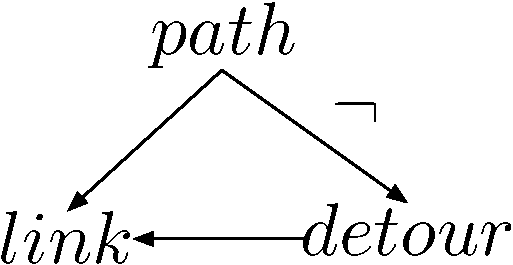
\includegraphics[scale=1]{figures/dependency-graph}
\caption{\label{ch:p2:fig:dependency}Dependency graph for predicates 
appearing in Figure~\ref{ch:p2:fig:negation}.}
\end{center} 
\end{figure*}

We can obtain the correct deductions by simply evaluating rule~\ol{R5} first.
Such an ordering of predicate evaluations forms the basic idea behind
stratified Datalog.  Before we get to that definition, lets first understand
how the dependencies of a Datalog program are represented graphically.
Figure~\ref{ch:p2:fig:dependency} contains the dependency graph for the predicates
appearing in the rules of Figure~\ref{ch:p2:fig:negation}. Constructing this graph
is a straightforward application of the following two rules.
\begin{enumerate}
  \ssp
  \item Add $p \rightarrow q$ dependency if there is a rule with head predicate $p$ and subgoal $q$.
  \item Add $p \rightarrow q$ dependency labeled $\neg$ if there is a rule with head predicate $p$ and negated subgoal $q$.
\end{enumerate}
From Figure~\ref{ch:p2:fig:negation}, rule~\ol{R4} forms the $path \rightarrow
link$ and $path \rightarrow detour$ dependencies, while rule~\ol{R5} supplies the
$detour {\neg \atop \rightarrow} link$ negated dependency. 

The stratum of an IDB predicate $p$ is defined to be the largest number of
negations ($\neg$) along any path involving predicate $p$.  The dependency graph
in Figure~\ref{ch:p2:fig:dependency} places predicates \ol{detour} and
\ol{link} in the lowest stratum~$0$, while the \ol{path} predicate is in
stratum~$1$.  If all IDB predicates have a finite stratum, then the Datalog
program is {\emph stratified}.  If any IDB predicate has an $\infty$ stratum,
then the program is unstratified.  An IDB predicate is assigned an $\infty$
stratum if it defines a negated subgoal on a path that contains a cycle (due
to arbitrary recursion).

We evaluate a stratified Datalog program using the seminaive algorithm of
Figure~\ref{ch:p2:fig:seminaive} but with a slight twist -- we topologically
sort the IDB predicates (in $\delta IDB$) by their assigned stratum, and follow
this order in the loop.  This order ensures that if the program is stratified
then any negated subgoal (e.g., \ol{detour}) has already had its relation fully
evaluated first.  The result of this evaluation is called a {\emph stratified
model}~\footnote{We note that the notion of stratified Datalog has nothing to
do with the termination of a Datalog program.  An unstratified Datalog program
that is ``safe'' is guaranteed to terminate.  The issue here is whether the
result produced by that evaluation is consistent with the programmer's
intent.}.

We revisit the notion of stratified Datalog throughout this thesis.  It turns
out that the P2 system does not supported stratified Datalog, which slightly
complicated the (\OVERLOG) program rules described in Chapters~\ref{ch:evita},
\ref{ch:magic} and~\ref{ch:opt}.  Fortunately, there is another class of {\emph
locally stratified} Datalog programs that ``make sense'' on certain data.

\subsection{Local Stratification}

The definition of stratified Datalog is based on cycles through negations in
the dependency graph of a collection of rules.  An extension to this definition
is a class of locally stratified programs.  These programs are not necessary
stratified according the their rules, but they are stratified when we
instantiate those rules with a specific collection of data.  Many of the
programs presented in this thesis fall into the class of locally stratified
rules.

\begin{figure*}
\ssp
\begin{boxedminipage}{\linewidth}
{\bf link}(``node1'', ``node2'', 1). \\
{\bf link}(``node2'', ``node3'', 1). \\
\\
R1 {\bf path}(X, Y, {\em cons}(X, Y), C) :- \\
\datalogspace {\bf link}(X, Y, C). \\
\\       
R2 {\bf path}(X, Z, {\em cons}(P1, P2), $C1+C2$) :- \\
\datalogspace {\bf link}(X, Y, C1), {\bf shortestPath}(Y, Z, P2, C2), \\
\datalogspace $f\_contains(X,\ P2)\ ==\ false$. \\ 

R3 {\bf minCostPath}(X, Y, min$<$C$>$) :-  \\
\datalogspace {\bf path}(X, Y, P, C).

R4 {\bf shortestPath}(X, Y, P, C) :- \\
\datalogspace {\bf minCostPath}(X, Y, C), {\bf path}(X, Y, P, C).\\

\end{boxedminipage}
\caption{\label{ch:p2:fig:datalogSP}Shortest path variant of Figure~\ref{ch:p2:fig:datalogPath}.}
\end{figure*}

Consider the variant of the path program in Figure~\ref{ch:p2:fig:datalogSP},
which modifies rule~\ol{R2} to formulate new paths from the \ol{shortestPath} 
relation, rather than the \ol{path} relation.  Two extra rules \ol{R3} and \ol{R4} are used to
derive the shortest path from the \ol{path} relation.  Rule~\ol{R3} selects the
minimum cost path from $X$ to $Y$, and rule~\ol{R4} selects the actual minimum
path based on the minimum cost metric.

\begin{figure*} 
\ssp
\begin{center}
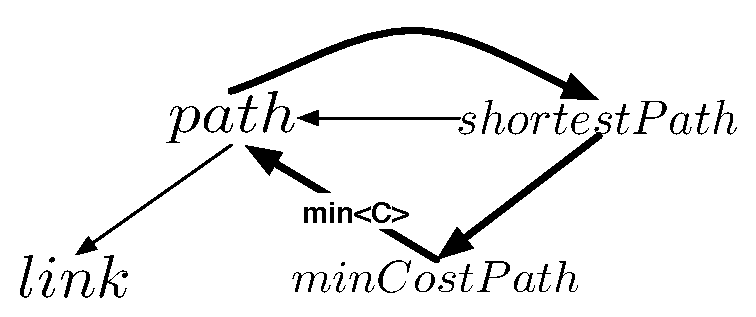
\includegraphics[scale=1]{figures/dependency-graph2}
\caption{\label{ch:p2:fig:dependency2}Dependency graph for predicates 
appearing in Figure~\ref{ch:p2:fig:datalogSP}. A cycle through an aggreagation
appears in bold. }
\end{center} 
\end{figure*}

The dependency graph for this program is shown in
Figure~\ref{ch:p2:fig:datalogSP}.  As shown, this program is not stratified
since there is a recursive path in the rule dependency graph that traverses an
aggregation.  Like negations, aggregations impose stratification boundaries.
Intuitively, we need to derive all \ol{path} tuples before we can identify the
one that is the minimum cost.  As a result, the Datalog program in
Figure~\ref{ch:p2:fig:datalogSP} is not stratified.

It is however locally stratified.  Assume that this program is evaluated using
the algorithm describe in Figure~\ref{ch:p2:fig:seminaive}.  The bottom-up
evaluation will start by deriving all paths of length $1$ using rule~\ol{R1},
then using rule~\ol{R2} to derive paths of length $2, 3, \cdots$ (fully, in
that order) until no such paths exist.  As a result of this {\emph derivation}
order, our {\bf min} aggregation will never see a fact (i.e., a \ol{path}
tuple) that disputes and earlier deduction.  That is, the naive and seminaive
evaluations derive \ol{path} tuples of length $k$ from {\bf all} \ol{path}
tuples of length $k-1$, and therefore it will not discover a path of length $j
> k$ with a lower cost~\footnote{This assumes that the cost of a \ol{path}
tuple is proportional to it's length i.e., the triangle inequality.}.

Many of the programs described in this thesis are not stratified, and of those,
all are locally stratified.  For example, the System R rules presented in
Chapter~\ref{ch:opt} perform a {\bf min} aggregation on the cost metric of a
query plan.  This is used to select the ``best plan'' among the set of
equivalent plans in a given level (plan size) of the System R dynamic program.
The ``best plan'' is then recursively used to construct new plans, containing
an extra predicate, for the next dynamic programming level.  Since adding an
extra predicate to a query plan can only increase its cost ({\emph principle of
optimality}), and we fully explore a level bottom-up, this optimization is locally
stratified.


\section{\OVERLOG: Our first look}
\label{ch:p2:sec:overlog}

\OVERLOG marks a new beginning for the Datalog recursive query language, where
distribution through data partitioning takes center stage.  Like Datalog, an
\OVERLOG~{\em program} consists of a set of deduction {\em rules} that define
the set of tuples that can be derived from a base set of tuples called {\em
facts}.  Each rule has a {\em body} on the right of the \texttt{:-} divider,
and a {\em head} on the left; the head represents tuples that can be derived
from the body.  The body is a comma-separated list of {\em terms}; a term is
either a {\em predicate} (i.e., a relation), a {\em condition} (i.e., a
relational selection) or an {\em assignment}~\footnote{\OVERLOG's assignments
are strictly syntactic replacements of variables with expressions; they are
akin to ``\#define'' macros in C++.}.  An example \OVERLOG program is shown in
Figure~\ref{ch:p2:fig:overlogSP}.  \OVERLOG introduces some notable extensions
to Datalog, which we describe before presenting the P2 runtime.

\begin{figure*}
\ssp
\begin{boxedminipage}{\linewidth}
{\bf materialize}(link,infinity,infinity,keys(1,2)). \\
{\bf materialize}(path,infinity,infinity,keys(1,2,3)).  \\
{\bf materialize}(shortestPath,infinity,infinity,keys(1,2,3)). \\

{\bf link}(``localhost:10000'', ``localhost:10001'', 1). \\
{\bf link}(``localhost:10001'', ``localhost:10002'', 1). \\

R1{\bf path}(@X, Y, P, C) :- \\
\datalogspace {\bf link}(@X, Y, C), P := f\_cons(X, Y). \\

R2 {\bf path}(@X,Z,P,C) :- \\
\datalogspace {\bf link}(@X, Y, C1), {\bf path}(@Y, Z, P2, C2), \\
\datalogspace $f\_contains(X,P2) == false$, \\
\datalogspace P := f\_cons(X,P2), C := C1 + C2. \\ 

R4 {\bf minCostPath}(@X, Y, a\_min$<$C$>$) :-  \\
\datalogspace {\bf path}(@X, Y, P, C). \\

R5 {\bf shortestPath}(@X, Y, P, C) :- \\
\datalogspace {\bf minCostPath}(@X, Y, C), {\bf path}(@X, Y, P, C).\\

Query {\bf shortestPath}(``localhost:10000'', Y, P, C).
\end{boxedminipage}
\caption{\label{ch:p2:fig:overlogSP}Shortest path program in \OVERLOG. \ol{a\_}
prefixes introduce aggregate functions and \ol{f\_} prefixes introduce
built-in functions.}
\end{figure*}

\subsection{Horizontal partitioning}

\OVERLOG's basic data model consists of relational tables that are partitioned
across distributed nodes in a network.  Each relation in an \OVERLOG rule must
have one attribute, whose variable is preceded by an ``@'' sign.  This
attribute is called the {\em location specifier} of the relation, and must
contain values in the network's underlying address space (e.g., IP addresses
for Internet settings, 802.13.4 addresses for sensor networks, hash-identifiers
for code written atop distributed hash tables, etc.).  Location specifiers
define the horizontal partitioning of the relation: each tuple is stored at the
address found in its location specifier attribute.  At a given node, we call a
tuple a {\em local tuple} if its location specifier is equal to the local
address.  Network communication is implicit in \OVERLOG: tuples must be stored
at the address in their location specifier, and hence the runtime engine has to
send some of its derived tuples across the network to achieve this physical
constraint.  Loo, et al.  provide syntactic tests to ensure that a set of rules
can be maintained partitioned in a manner consistent with its location
specifiers and network topology~\cite{loo-sigmod06}.


\subsection{Soft State and Events}

Associated with each \OVERLOG table is a ``soft-state'' lifetime that
determines how long (in seconds) a tuple in that table remains stored before it
is automatically deleted.  Lifetimes can vary from zero to $\infty$.
Zero-lifetime tables are referred to as {\em event} tables, and their tuples
are called \emph{events}; all other tables are referred to as {\em
materialized} tables.  \OVERLOG contains a \ol{materialize} declaration that
specifies the lifetime of a materialized table.  At any instant in time, at any
given node in the network, the contents of the local \OVERLOG ``database'' are
considered to be: (a) the local tuples in materialized tables whose lifetime
has not run out, (b) at most one local event fact across {\em all} event
tables, and (c) any derived local tuples that can be deduced from (a) and (b)
via the program rules.  Note that while (b) specifies that only one event fact
is considered to be live at a time per node, (c) could include {\em derived}
local events, which are considered to be live simultaneously with the event
fact.  This three-part definition defines the semantics for a single P2 node at
a snapshot in time.  P2 has no defined semantics across time and space (in the
network); we describe the relevant operational semantics of the prototype in
Section~\ref{ch:p2:sec:p2}.
     
\subsection{Deletions and Updates}

\OVERLOG, like SQL, supports declarative expressions that identify tuples to be
deleted, in a deferred manner after a fixed point is achieved. To this end, any
\OVERLOG rule in a program can be prefaced by the keyword \ol{delete}.  The
program is run to fixpoint, after which the tuples derived in {\tt delete}
rules -- as well as other tuples derivable from those -- are removed from
materialized tables before another fixpoint is executed.  It is also possible
in \OVERLOG to specify updates, but the syntax for doing so is different.
\OVERLOG's {\tt materialize} statement supports the specification of a primary
key for each relation.  Any derived tuple that matches an existing tuple on the
primary key is intended to {\em replace} that existing tuple, but this
replacement happens through an insertion and a deletion: the deduction of the
new tuple to be inserted is visible within the current fixpoint, whereas the
deletion of the original tuple is deferred until after the fixpoint is computed.

\subsection{A Canonical Example}
\label{ch:p2:sec:declnet}

To illustrate the specifics of \OVERLOG, we describe the shortest paths example
in Figure~\ref{ch:p2:fig:overlogSP}, which is similar to that
of~\cite{loo-sigmod06}, but with fully-realized \OVERLOG syntax that runs in
P2.  The three \ol{materialize} statements specify that \ol{link}, \ol{path}
and \ol{bestpath} are all tables with $\infty$ lifetime and $\infty$ storage
space\footnote{The third argument of P2's table definition optionally specifies
a constraint on the number of tuples guaranteed to be allowed in the relation.
The P2 runtime replaces tuples in ``full'' tables as needed during execution;
replaced tuples are handled in the same way as tuples displaced due to
primary-key overwrite.}.  For each table, the positions of the primary key
attributes are noted as well.  Rule \ol{r1} can be read as saying ``if there is
a link tuple of the form \ol{(X,Y,C)} stored at node \ol{X}, then one can
derive the existence of a path tuple \ol{(X,Y,P,C)} at node \ol{X}, where
\ol{P} is the output of the function \ol{f\_cons(X,Y)} -- the concatenation of
\ol{X} and \ol{Y}.'' Note that rule \ol{r1} has the same location specifiers
throughout, and involves no communication.  This is not true of the recursive
rule \ol{r2}, which connects any \ol{link} tuple at a node \ol{X} with any path
tuple at a neighboring node \ol{Y}, the output of which is to be stored back at
\ol{X}.  As described in the earlier work on
P2~\cite{loo-sigcomm05,loo-sigmod06} such rules can be easily rewritten so that
the body predicates all have the same location specifier; the only
communication then is shipping the results of the deduction to the head
relation's location specifier.  We declaratively describe this simple 
localization ``rewrite'' in Chapter~\ref{ch:evita}.

\section{The P2 Runtime Engine}
\label{ch:p2:sec:p2}

The P2 runtime is a dataflow engine that was based on ideas from relational
databases and network routers; its scheduling and data hand-off closely
resemble the Click extensible router~\cite{click-tocs}.  Like Click, the P2
runtime supports dataflow {\em elements} (or ``operators'') of two sorts:
pull-based elements akin to database iterators~\cite{graefe-survey}, and
push-based elements as well.  As in Click, whenever a pull-based element and a
push-based element need to be connected, an explicit ``glue'' element (either a
pull-to-push driver, or a queue element) serves to bridge the two.  More
details of this dataflow coordination are presented in the original P2
paper~\cite{p2:sosp}.  Here we focus on the dataflow architecture
(Section~\ref{ch:p2:sec:dataflow}), which affects the language semantics, and
the individual processing elements (Section~\ref{ch:p2:sec:dataflow_elements}).

\subsection{Dataflow Architecture}
\label{ch:p2:sec:dataflow}

\begin{figure*} 
\ssp
\begin{center}
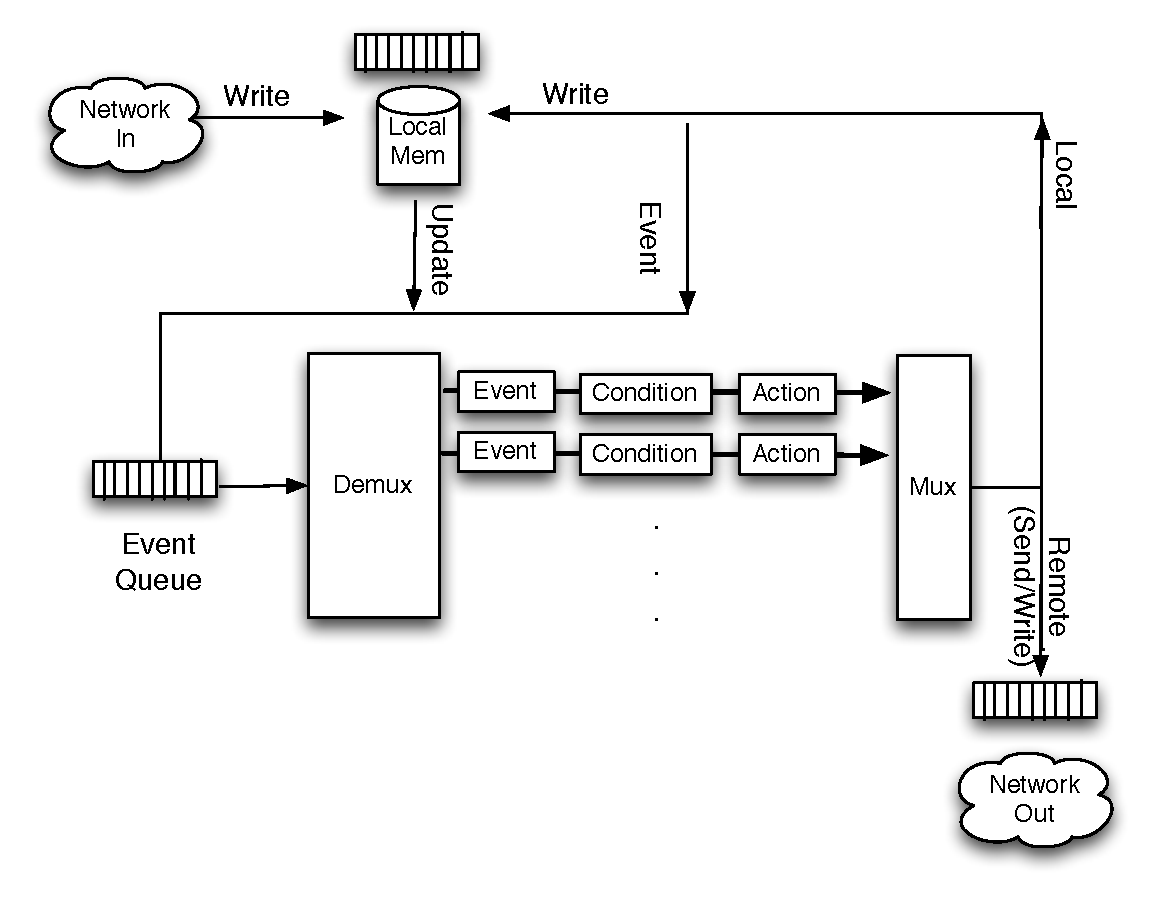
\includegraphics[scale=0.6]{figures/p2-arch}
\caption{\label{ch:p2:fig:dataflow}P2 Dataflow Architecture.}
\end{center} 
\end{figure*}

The P2 architecture consists of a dataflow of processing elements and queues,
and a single driver loop.  Figure~\ref{ch:p2:fig:dataflow} provides a high
level view of this architecture, which contains three queuing elements.  The
\ol{event} queue represents the primary input queue, which contains the
``working set'' of tuples that the system is currently processing.  The
\ol{netin} and \ol{localmem} secondary queues feed the main event queue with
tuples when none currently exist in it.

The P2 architecture contains three output queues that hold the tuples derived
from the rule engine.  The choice of which queue a tuple is added to depends on
the value of the location attribute.  If the tuple's location is local to the
current P2 instance, and its lifetime is greater than zero, then it will be
added to the \ol{localmem} queue.  If the tuple is remote, then it is added to
the \ol{netout} queue.  The third output queue is the \ol{event} queue.  All
local tuples that have a zero-lifetime are directly added to the this queue.
This implementation decision exhibited a kind of ``mini-fixpoint'' (a side-effect 
unique to P2-\OVERLOG) that we refer to as a dataflow fixpoint, which
occurs when all tuples in the event queue have been drained.  We describe this
by example.

Assume a single tuple in the \ol{netin} input queue, and all other queues are
empty.  When the driver executes its ``pull-push'' element on the input of the
\ol{event} queue, it will dequeue the tuple in the \ol{netin} queue, write it
to the relevant local memory table, and add the result of that write operation
to the \ol{event} queue.  In an iterative loop, the driver will dequeue a
single tuple from the \ol{event} queue and ``route it'' to the processing
elements, which derives some number of new deductions.  If any of those
deductions contain local tuples with a zero lifetime, then they are reinserted
into the \ol{event} queue.  The driver loop continues to process tuples from
the \ol{event} queue until it is again empty.  At this point, it declares a
dataflow fixpoint, which triggers a flush of the ``insertion'' writes from the
\ol{localmem} queue.  If no ``insertion'' tuples exist then a flush of the
``deletion'' tuples occur, and the corresponding deletion events are added to
the \ol{event} queue, before the process repeats, this time treating deductions
as further deletions.

After all insertion and deletion tuples have been processed by the initial
\ol{netin} input tuple, the system declares a global fixpoint, which is
semantically equivalent to a Datalog fixpoint.  On a global fixpoint, the
driver loop will flush all tuples in the \ol{netout} queue, triggering a
transfer of those tuples to the corresponding P2 instances spanning the
network.  The driver loop then returns to the \ol{netin} queue for the next
tuple to process.

From this perspective, the P2 runtime looks quite a bit like an
Event-Condition-Action (ECA) system with a dataflow underneath: events are
provided by the clock and network, conditions are checked via dataflow
processing elements, and actions take the form of sending/receiving network
messages and updates to relational state.  These actions are performed at
well-defined moments, with provably verifiable language
semantics~\cite{boon-thesis}.  The ``event'' portion of ECA is implemented by
the driver loop and routed to the ``conditions'' by the \ol{demux} element in
Figure~\ref{ch:p2:fig:dataflow}.  The event loop of P2 defines the notion of a
{\emph floating} EDB, that at a given instance of time, consists of the single
tuple at the head of the \ol{netin} queue.  This sole tuple is the input to the
``current'' Datalog fixed point.  Next, we describe the elements that implement
the {\emph condition} and {\emph action} processing logic.

\subsection{Dataflow Elements} 
\label{ch:p2:sec:dataflow_elements}

The set of elements provided in P2 includes a suite of operators familiar from
relational query engines: selection, projection, and in-memory indexes.  These
operators are strung together to implement the logical {\emph condition} of the 
processing loop.  P2 supports joins of two relations in a manner similar to the
symmetric hash join: it takes an arriving tuple from one relation, inserts it
into an in-memory table for that relation, and probes for matches in an access
method over the other relation (either an index or a scan).  The work described
in Chapter~\ref{ch:evita} extended this suite to include sorting and
merge-joins, which allowed us to explore some traditional query optimization
opportunities and trade-offs (Chapter~\ref{ch:opt}).

P2 consists of exactly two logical {\emph actions}: a local database write and
a network send.  We first describe the details of behind a database write.  An
\ol{event} tuple is modeled as transient database write, and therefore its
action is the reinsertion into the \ol{event} queue.  P2 does not currently
have support for persistent storage, beyond the ability to read input streams
from comma-separated-value files.  Its tables are stored in memory-based
balanced trees that are instantiated at program startup; additional such trees
are constructed by the planner as secondary indexes to support predicate join
attributes.  A write to the database is applied to the memory-based table, and
a relevant (insert/delete) \ol{event} is enqueued into the \ol{localmem} queue.

The action for a remote output tuple is to simply enqueue it on the \ol{netout}
queue.  When this queue is eventually flushed by the driver loop, all tuples in
it are sent over the network prior to the next fixpoint iteration.  As part of
the same dataflow, P2 provides a number of elements used for networking, which
handle issues like packet fragmentation and assembly, congestion control,
multiplexing and demultiplexing, and so on; these are composable in ways that
are of interest to network protocol designers~\cite{condie-hotnets05}.  The
basic pattern that the reader should assume is that each P2 node has a single
IP port for communication, and the dataflow graph is ``wrapped'' in elements
that handle network ingress with translation of packets into tuples, and
network egress with translation of tuples into packets.

%\subsubsection{Driver Loop}

%We now describe the complete control flow in the P2 runtime.  As mentioned
%above, it is driven by a fairly traditional event loop that responds to any
%network (or timer) event by invoking an appropriate dataflow segment to handle
%the event.
%
%The basic control loop in P2 works as follows:
%\begin{CompactEnumerate}
%    \item An event is taken from the system input queue, corresponding to a single newly-arrived tuple, which is either an {\em insert} tuple (i.e., the result of a normal deduction) or a {\em delete} tuple (the result of a \ol{delete} rule or a primary-key update).  We will refer to this tuple as the {\em current tuple}.
%    \item The value of the system clock is noted in a variable we will call the {\em current time}.  This is the time that will be used to determine the liveness of soft-state tuples.  
%    %(Note that any event tuples that arrived previously will no longer be live in any event table, which guarantees the single-event semantics described above.)
%    \item The current tuple is, logically, appended to its table.
%    \item If the current tuple is an insert tuple, the dataflow corresponding to the \OVERLOG program is initiated and run to a local fixpoint following traditional Datalog semantics, with the following exception: during processing, any non-local derived tuples are buffered in a {\em send queue}, as are any derived tuples to be deleted.
%    \item If, instead, the current tuple is a delete tuple, the dataflow
%    is run to a local fixpoint, but newly-derived local tuples
%    (including the current tuple) are copied to a {\em delete queue},
%    and newly-derived non-local tuples are marked as delete tuples
%    before being placed in the send queue so as to cascade the deletions
%    to remote nodes' databases.
%    \item All tuples in the delete queue are deleted from their associated tables, and the delete queue is emptied.
%    \item The send queue is flushed across the network, with any local updates inserted into the local input queue.
%\end{CompactEnumerate}

%Unlike Datalog, \OVERLOG must run in the continuous processing context of
%networking, over streams of tuples representing system events.  This inherently
%requires more than the single computation of a fixpoint as described in the
%Datalog literature.  P2 has modified its handling of this issue since the
%initial paper~\cite{p2:sosp}.  P2 nests a fairly traditional declarative
%Datalog fixpoint execution within an operationally defined local event loop at
%each node.  An input queue is kept at each P2 node, to hold tuples that
%correspond to network messages and clock interrupts.  Each tuple in the queue
%is tagged with the name of a relation in the schema of the Datalog database.
%The loop begins by noting the local wall-clock time, and deleting from all
%tables any tuples whose soft-state lifetime has expired; this includes event
%tuples from the previous iteration of the loop.  At that point, a tuple is
%dequeued from the input queue and inserted into its associated table.  At that
%point, the \OVERLOG program is run to fixpoint atomically, nearly as if it were
%a traditional single Datalog program.  One exception to traditional Datalog is
%the handling of derived tuples with remote location specifiers; these are
%placed directly into network queues for subsequent processing.  Another
%exception involves rules that have {\em actions} in the head -- these actions
%can be table insertion or deletion; derived tuples in such rules are also
%enqueued for subsequent processing.  When fixpoint is reached, the queued
%network messages are sent to their destinations, and the table actions are
%carried out on the database.  This completes one iteration of the event loop.


\section{Summary}
\label{ch:p2:sec:summary}

While ostensibly a network protocol engine, architecturally P2 resembles a
fairly traditional shared-nothing parallel query processor, targeted at both
stored state and data streams.  The P2 runtime at each node consists of a
compiler---which parses programs, optimizes them, and physically plans them---a
dataflow executor, and access methods.  Each P2 node runs the same query
engine, and, by default, participates equally in every ``query.'' In parallel
programming terms, P2 encourages a Single-Program-Multiple-Data (SPMD) style
for parallel tasks, but also supports more loosely-coupled (MPMD) styles for
cooperative distributed tasks, e.g.  for communications among clients and
servers.


% \jmh{This is probably too long.  Also, we need to purge text that was recycled from SOSP.  }
% The design of P2 was inspired by prior work in both databases and
% networking. It is based in large part upon a
% side-by-side comparison between the PIER peer-to-peer query
% engine~\cite{pier-cidr05} and the Click router~\cite{click-tocs}. Like
% PIER, P2 can manage structureddata tuples flowing through a broad
% range of query processing elements, which may accumulate significant
% state and perform substantial asynchronous processing.  Like Click, P2
% stresses high-performance transfers of data units, as well as dataflow
% elements with both ``push'' and ``pull'' modalities. 
% 
% At a coarse grain, P2 in its current state consists of (1) an \OVERLOG
% parser, (2) an Planner that translates \OVERLOG to a runtime dataflow
% plan, and (3) a runtime plan executor.  The
% life of a query is simple: the query is parsed into an internal
% representation, the planner constructs a corresponding dataflow graph
% of elements, and the graph is executed by the runtime until it is
% canceled.  We proceed to overview the components bottom-up; more
% details are given in the P2 SOSP paper~\cite{p2:sosp}.
% 
% Processing in P2 is handled with a dataflow model inspired by Click
% and PIER.  As in Click, nodes in a P2 dataflow
% graph can be chosen from a set of C++ objects called
% \textit{elements}.  In database systems these are often called
% \textit{operators}, since they derive from logical operators in the
% relational algebra.  Elements have some number of input and output
% \emph{ports}.  An arc in the dataflow graph is represented by a
% binding between an output port on one element and an input port on
% another.  Tuples arrive at the element on input ports, and elements
% emit tuples from their output ports. Handoff of a tuple between two elements takes one
% of two forms, \emph{push} or \emph{pull}, determined when the elements
% are configured into a dataflow graph.   
% 
% P2 provides a number of built in dataflow elements that allow it to
% implement networking and query processing logic.  This includes
% elements for the streaming relational query operators found in most
% database systems, e.g., selection, projection, join, and aggregation.
% It also includes networking elements responsible for socket handling,
% packet scheduling, congestion control, reliable transmission, data
% serialization, and dispatch.  P2 has elements to store incoming tuples in tables, 
% iteratively emit tuples in a table matching a filter expression, and {\em listener}
% elements that are notified whenever a tuple is added or deleted from a
% table. Finally, like Click, P2 includes a collection of general-purpose
% ``glue'' elements, such as a queue, a multiplexer, a round-robin
% scheduler, etc.
% 
% Storage in P2 is currently via a main-memory relational Table
% implementation, named using unique IDs that can be shared between
% different queries and/or dataflow elements.  In-memory indices
% (implemented using standard balanced binary trees) can be attached to
% attributes of tables to enable quick equality lookups.  The current
% in-memory implementation serves the system requirements for implementing
% network overlays and streaming query applications, all of which tend
% to expire tuples from memory rather than accumulating them
% indefinitely.  P2's event-driven, run-to-completion model obviates the
% need for locking or transaction support, and relatively simple indices
% suffice to meet performance requirements.  We plan additional
% table implementations that use stable storage for persistent data
% storage; that engineering task is relatively straightforward, but not
% within the scope of this paper.
% 
